\documentclass
[
a4paper,															%Papierformat
11pt,																%Schriftgröße
twoside=true,														%Zweiseitig
openright,															%Neues Kapitel immer auf der rechten Seite
titlepage,															%Titelseite
headinclude,														%Seitengröße auch bei Kopfzeile
numbers=noenddot,													%Bei Kapiteln keine abschließenden Punkte
listof=numbered,													%Listingsverzeichnis
bibliography=totocnumbered,											%Literaturverzeichnis
]
{scrbook}															%Dokumenttyp
\usepackage[ngerman]{babel}											%Deutsch
\usepackage[bottom=1in,inner=1in,outer=20mm,top=20mm]{geometry}		%Ganze Seite
\usepackage{emptypage}												%Leere Seiten ohne Kopf und Fußzeile
\usepackage[headsepline]{scrlayer-scrpage}							%Kopf und Fußzeile
\pagestyle{scrheadings}												%Nummerierung in der Kopfzeile
\clearscrheadfoot													%Kopf und Fußzeile löschen
\rehead{\headmark}													%Kapitelname auf der geraden Seite innen
\ohead[\pagemark]{\pagemark}										%Seitennummerierung
\lohead{}															%Name auf der ungeraden Seite innen
\renewcommand*{\chapterpagestyle}{scrheadings}						%Kopf und Fußzeile auf Seiten mit Überschriften anders
\usepackage{graphicx}												%Bilder
\usepackage{caption}												%Tabellen Listings und Figuren mit beschriftung im Verzeichnissen
\usepackage[T1]{fontenc}											%Outputencoding
\usepackage{float}													%Plazierung von Floats (Bilder Tabellen)
\usepackage[utf8]{inputenc}											%UTF8
\usepackage{wrapfig}												%Textumfluss von Bildern, die nicht die ganze Seite Brauchen
\usepackage{setspace}												%Zeilenabstand
\usepackage{listings}												%Listings (=Code)
\usepackage{times}													%Schriftart Times Roman
\usepackage{courier}												%Schriftart Courier
\usepackage{multirow}												%Bessere Tabellenformatierung
\usepackage{array}													%Bessere Tabellenformatierung
\usepackage{xcolor}													%Farben für Codehighlighting oder ähnliches
\usepackage{appendix}												%Anhang Titelseite
\usepackage{tabularx}												%Bessere Tabellen
\usepackage{jurabib}												%Zitierung
\usepackage[bookmarks]{hyperref}									%Automatische Lesezeichen
\usepackage{ucs}
\usepackage{amsmath,amssymb,amstext}
\usepackage{multicol}
\usepackage{latexsym}
\usepackage{textcomp}


\setlength{\parindent}{0em}											%Einrücken

\subject{
\includegraphics[scale=0.7]{logoMecha.png}}
\title{Pferdeführanlage}
\subtitle{HTBLA Kaindorf an der Sulm\\Grazer Straße 202, A-8430 Kaindorf an der Sulm\\Ausbildungsschwerpunkt Mechatronik und Automatisierungstechnik}
\author{Stefan Christian Ornik \and Dominik Roland Riegelnegg \and Lukas Freyler \and Fabio Pölzl}
\date{Abgabedatum: \today{}}
\publishers{Betreut von:\\Dipl.-Ing Wolfgang Mader \\ Dipl.-Päd Otto Schuller \\ Dipl.-Ing. Manfred Steiner \\ Dipl.-Ing. Werner Harnisch}
\begin{document}													%Dokumentbeginn
\onehalfspace														%Zeilenabstand
\maketitle															%Titelseite
\setcounter{tocdepth}{5}											%Tiefe der Überschriften
\setcounter{secnumdepth}{5}											%Nummerierungstiefe der Überschriften
%Java
%Model from netbeans
\definecolor{java_net_comment}{rgb}{0.586,0.586,0.586}
\definecolor{java_net_keyword}{rgb}{0,0,0.898}
\definecolor{java_net_string}{rgb}{0.805,0.480,0}
\definecolor{java_net_preprocessor}{rgb}{0,0.597,0}
\definecolor{codeBackGray}{gray}{0.98}

\lstdefinestyle{java}{ 																					%define java style
  language=Java,                 																		% the language of the code
  backgroundcolor=\color{codeBackGray},   																% choose the background color
  basicstyle=\fontencoding{T1}\fontfamily{courier}\fontseries{m}\selectfont\footnotesize,    			% the size of the fonts that are used for the code
  breakatwhitespace=false,         																		% sets if automatic breaks should only happen at whitespace
  breaklines=true,                 																		% sets automatic line breaking
  captionpos=b,                    																		% sets the caption-position to bottom
  commentstyle=\color{java_net_comment},    															% comment style
  escapeinside={(}{)},          																		% if you want to add LaTeX within your code
  extendedchars=true,             		 																% lets you use non-ASCII characters; for 8-bits encodings only, does not work with UTF-8
  frame=none,%single,	                   																% adds a frame around the code
  framexleftmargin=8mm,																					%include numbers into the frame
  keepspaces=true,                																		% keeps spaces in text, useful for keeping indentation of code (possibly needs columns=flexible)
  keywordstyle=\color{java_net_keyword},       															% keyword style
  deletekeywords=          																				% if you want to delete keywords from the given language
 {}, 
  otherkeywords={},           																			% if you want to add more keywords to the set
  numbers=left,                    																		% where to put the line-numbers; possible values are (none, left, right)
  numbersep=8pt,                   																		% how far the line-numbers are from the code
  numberstyle=\fontencoding{T1}\fontfamily{courier}\fontseries{m}\selectfont\footnotesize,				% the style that is used for the line-numbers
  rulecolor=\color{black},         																		% if not set, the frame-color may be changed on line-breaks within not-black text (e.g. comments (green here))
  showspaces=false,                																		% show spaces everywhere adding particular underscores; it overrides 'showstringspaces'
  showstringspaces=false,          																		% underline spaces within strings only
  showtabs=false,                  																		% show tabs within strings adding particular underscores
  stepnumber=1,                    																		% the step between two line-numbers. If it's 1, each line will be numbered
  stringstyle=\color{java_net_string},     																% string literal style
  tabsize=2,	                   																		% sets default tabsize to 2 spaces
  title=\lstname,                  		 																% show the filename of files included with
}

\newcommand{\inlinecode}[2]{\colorbox{editorGray}{\lstinline[language=#1]$#2$}}
\frontmatter												%Seitennumerierung
\pagenumbering{Roman}										%Römische Zahlen
\addtocounter{page}{2}

\newcommand{\doublesignature}[2]{%
  \parbox{\textwidth}{
    \hfill
    \parbox{7cm}{
      \centering
      \rule{6cm}{1pt}\\
      #1
    }
    \parbox{7cm}{
      \centering
      \rule{6cm}{1pt}\\
      #2
    }
  }
  \mbox{}\\
  \mbox{}\\
  \mbox{}\\
  \mbox{}\\
}

\vspace*{20pt}

\section*{Eidesstattliche Erklärung}
\label{sec:eidestattliche-erklaerung}
Ich erkläre an Eides statt, dass ich die vorliegende Arbeit selbstständig verfasst, andere als die angegebenen
Quellen/Hilfsmittel nicht benutzt und die den benutzten Quellen wörtlich und inhaltlich entnommenen
Stellen als solche kenntlich gemacht habe.\\
\\
Arnfels, am 05. April 2018\\

\vskip 2cm

\doublesignature{Lukas Freyler}{Stefan Ornik}
\doublesignature{Fabio Pölzl}{Dominik Riegelnegg}

\vskip 5cm

\clearpage

\newpage
\thispagestyle{empty}
\mbox{}

\clearpage

\section*{Danksagung}
\label{sec:danksagung}
An dieser Stelle möchten wir uns bei allen bedanken, die uns im Rahmen der Diplomarbeit unterstützt und betreut haben.\\
\\
Besonders bedanken möchten wir uns bei unseren Betreuern, Dipl.-Ing. Werner Harnisch, Dipl.-Ing. Wolfgang Mader, BEd. Otto Schuller
und Dipl.-Ing. Manfred Steiner für die fachliche Unterstützung während dieser Arbeit.

\newpage

\section*{Zusammenfassung}
\label{sec:zusammenfassungMain}

Das Hauptziel der Diplomarbeit ist es, Pferden mehr Bewegung zu ermöglichen. In der freien Natur legen Pferde einige Kilometer am Tag zurück. Dies können die Pferde in den verschiedensten Reitställen nicht behaupten. Die Haltung eines Pferdes bringt viele Kosten mit sich. Da bleibt meistens nichts mehr für ein neues Trainingsgerät für die Pferde übrig. Als Nächstes kommt hinzu, dass manche Personen auch nicht die nötige Zeit haben, um neben der Pferdeführanlage zu stehen und den Betrieb zu überwachen. Dadurch ergeben sich verschiedene Punkte, um die Schwierigkeiten für den Besitzer zu minimieren: \\
Unser Ziel ist es eine automatisierte Anlage zu entwickeln, welche einfach über eine Android Applikation zu steuern ist. Da die Anlage auch an heißen Tagen betrieben wird, wurde eine Kühlung für die Pferde auf die Liste der Abarbeitungspunkte gesetzt. Die Erfrischung soll mittels Sprühregen realisiert werden, damit die Pferde bei heißen Temperaturen eine Abkühlung bekommen können. Der Benutzer kann bis zu vier Pferde innerhalb der Anlage positionieren und diese starten. Die Zeit und die Geschwindigkeit der Pferdeführanlage soll er selbst auswählen können. Als letzten Punkt soll es eine Videoübertragung zur Android Applikation geben, damit der Benutzer jederzeit einen Blick auf die Anlage werfen kann, ob noch alles in Ordnung ist.  \newline{}
 
Was sind nun die wichtigsten Punkte von unserer Anlage?\\

\begin{itemize}
\item{Automatisierte Anlage}
\item{Platz für vier Pferde gleichzeitig}
\item{Android Applikation um die Anlage zu steuern}
\item{Videoüberwachung, die Bestandteil der Applikation ist}
\item{Einfache Bedienung}
\item{Geschwindigkeit und Zeit sollen individuell konfigurierbar sein} 
\item{Sprühregen zur Abkühlung der Pferde}
\item{Langlebig}
\end{itemize}

\newpage

\section*{Abstract}
\label{sec:abstractIntroduction}

The primary goal of this thesis is to enable horses more movement. Horses travel many kilometers a day in the case they live in the wildlife. Horses which are the most time of their life inside the stable are not able to do so. Moreover, keeping those animals implicates a lot of costs. As a result there is not any money left for a new training device. Another difficult is, that the keepers of the animals do not have the time required to stand by the horse exerciser and control the system. \\

This thesis wants to find ways to minimize those problems. The aim of the thesis is to develop an automated system which can be easily controlled by an Android application. The program should allow the user to compile a program for the horses. Because of the reason, that the horse exerciser is also going to operate during hot days, one mayor point is to develop a cooling system for the horses. If the user wants to train some horses, he has to place up to four horses inside the horse exerciser. Then he is able to start the system. He should also be able to set the operating time and speed of the horse exerciser. As a final step, as the system is video controlled, the user can check on the app, if everything is okay. \newline{}

What are the primary goals of the horse exerciser?\\

\begin{itemize}
	\item{automated unit}
	\item{capacity for up to four horses simultaneously}
	\item{Android application to control the system}
	\item{video control which is available inside the app}
	\item{easy handling}
	\item{speed and time should be able to be adapted individually}
	\item{light drizzle to cool down the horses}
	\item{persistent}
\end{itemize} 


\clearpage

\newpage
\thispagestyle{empty}
\mbox{}

\clearpage

\subsection*{Gender Erklärung}
\label{sec:gender-erklaerung}
Aus Gründen der besseren Lesbarkeit wird in dieser Arbeit die Sprachform des generischen Maskulinums angewendet. Es wird an dieser Stelle darauf hingewiesen, dass die ausschließliche Verwendung der männlichen Form geschlechtsunabhängig verstanden werden soll.

\subsection*{Über dieses Dokument}
\label{sec:ueber-dokument}
Diese Arbeit wurde in \LaTeX{} verfasst. Diese Art der Dokumentation bietet gegenüber den normalen Textverarbeitungen gewisse Vorteile hinsichtlich der Formatierung und des Einbindens von Grafiken. Auch Formeln können sehr einfach und effizient angegeben werden.

\clearpage

\newpage
\thispagestyle{empty}
\mbox{}

\clearpage

\section*{Projektteam}
\label{sec:projektteam}

\subsection*{Lukas Freyler}
\begin{wrapfigure}[10]{l}{0.5\textwidth}
\begin{center}
  
\includegraphics[width=0.35\textwidth]{fig/logoMecha}
\end{center}
\end{wrapfigure}
\mbox{}\\
\mbox{}\\
\textbf{Aufgabenbereich}:\\
\LaTeX{}\\
\textbf{Betreuer}:\\
Dipl.-Ing. Manfred Steiner
\mbox{}\\
\mbox{}\\
\mbox{}\\
\mbox{}\\
\mbox{}\\
\mbox{}\\

\subsection*{Stefan Ornik}
\begin{wrapfigure}[10]{l}{0.5\textwidth}
\begin{center}
  
\includegraphics[width=0.35\textwidth]{fig/logoMecha}
\end{center}
\end{wrapfigure}
\mbox{}\\
\mbox{}\\
\textbf{Aufgabenbereich}:\\
\LaTeX{}\\
\textbf{Betreuer}:\\
Dipl.-Ing. Wolfgang Mader
\mbox{}\\
\mbox{}\\
\mbox{}\\
\mbox{}\\
\mbox{}\\
\newpage

\subsection*{Fabio Pölzl}
\begin{wrapfigure}[10]{l}{0.5\textwidth}
\begin{center}
  
\includegraphics[width=0.35\textwidth]{fig/logoMecha}
\end{center}
\end{wrapfigure}
\mbox{}\\
\mbox{}\\
\textbf{Aufgabenbereich}:\\
\LaTeX{}\\
\textbf{Betreuer}:\\
Dipl.-Ing. Werner Harnisch
\mbox{}\\
\mbox{}\\
\mbox{}\\
\mbox{}\\
\mbox{}\\
\mbox{}\\

\subsection*{Dominik Riegelnegg}
\begin{wrapfigure}[10]{l}{0.5\textwidth}
\begin{center}
  
\includegraphics[width=0.35\textwidth]{fig/logoMecha}
\end{center}
\end{wrapfigure}
\mbox{}\\
\mbox{}\\
\textbf{Aufgabenbereich}:\\
\LaTeX{}\\
\textbf{Betreuer}:\\
BEd. Otto Schuller
\mbox{}\\
\mbox{}\\
\mbox{}\\
\mbox{}\\
\mbox{}\\
\newpage														%Datei importieren
\tableofcontents													%Inhaltsverzeichnis
\mainmatter															%Seitennummerierung
\chapter{Beispiele}

\section{Beispiel mit Code und Bildern}
\label{sec:beispiel}

\subsection{Code und Bilder}
\label{sec:code-bild}

\subsubsection{Sogar mit Textumfluss}
\label{sec:floating-text}

\paragraph{Bilder}\mbox{}\\

\begin{wrapfigure}{r}{0.6\textwidth}
\vspace{-30pt}
  \begin{center}
    
\includegraphics[width=0.55\textwidth]{fig/logoMecha}
  \end{center}
  \caption{Bild mit Textumfluss}
  \label{Bild mit Textumfluss}
  \vspace{-10pt}
\end{wrapfigure}

Hier muss Text stehen, sonst wird von unten alles verschoben. Sollte nicht genug Text vorhanden sein muss mit dem \textbackslash{}vspace\{\} Befehl das Format angepasst werden. Mit dem \textbackslash{}vspace\{\} Kommando muss solange herumgspielt werden, bis das Format passt. Sollte nicht genug Platz gebraucht werden, wird der \textbackslash{}wrapfigure\{\} Befehl auch weiter unten alles auf die halbe Seite verringern. Verweisen auf Sections, Bilder, etc. kann man mit dem Befehl \textbackslash{}ref\{\}. Hier ein Verweis auf die Tabellensection \ref{sec:tabelle}. Ein Verweis auf die Bilder \ref{Bild mit Textumfluss} und \ref{Bild über ganze Seitenbreite}.

\begin{figure}[H]
      
\includegraphics[width=1\textwidth]{fig/logoMecha}
      \caption{Bild über ganze Seitenbreite}
      \label{Bild über ganze Seitenbreite}
\end{figure}
\newpage

\paragraph{Code}\mbox{}\\
Hier muss Text stehen, sonst wird der Paragraph nicht angezeigt.\footnote{Fußnote mit URL.\\ \url{https://www.htl-mechatronik.at/}, (letzter Zugriff am 7.3.2018)} 

\begin{lstlisting}[style=java,caption=Java Codebeispiel]
package u04t;

import ue04.Bauteil;
import ue04.Kondensator;
import ue04.Placeable;
import ue04.PlaceableWiderstand;
import ue04.Spule;
import ue04.Widerstand;

// Kommentar mit Umlauten: ä, ö, ü, Ä, Ü, Ö, ß

/**
 *
 * @author sx
 */
public class Ue04
{
  public static void main (String[] args)
  {
    Widerstand r1 = new Widerstand(1000, 10);
    Kondensator c1 = new Kondensator(0.001, 1, r1.getCurrent());
    Spule l1 = new Spule (0.01, 5.4, c1.getCurrent());
    
    Bauteil [] bauteile = new Bauteil [4];
    bauteile[0] = r1;
    bauteile[1] = c1;
    bauteile[2] = l1;
    bauteile[3] = new PlaceableWiderstand(100, 2, 10, 12.3);
    
    double totalEnergy = 0.0;
    for (Bauteil b : bauteile)
    {
      System.out.print(b);
      if (b instanceof Placeable)
      {
        Placeable p = (Placeable)b;
        System.out.print(" x=" + p.getX() + "  y=" + p.getY());
      }
      System.out.println();
      
      totalEnergy += b.getEnergy();
    }
    System.out.println("Gesamtenergie: " + totalEnergy + "J");
    
  }
}

\end{lstlisting}
\newpage

\section{Tabellenbeispiel}
\label{sec:tabelle}

Tabelle \ref{Tabellenbeispiel} ist mit einem Onlinegenerator erzeugt, da Tabellen anstrengend sind.

\begin{table}[H]
\resizebox{0.5\textwidth}{!}{%
\begin{tabular}{|c|c|c|c|c|}
\hline
\textit{\textbf{1}} & \textit{\textbf{2}}  & \textit{\textbf{3}}  & \textit{\textbf{4}}  & \textit{\textbf{5}}  \\ \hline
\textit{\textbf{2}} & \textit{\textbf{4}}  & \textit{\textbf{6}}  & \textit{\textbf{8}}  & \textit{\textbf{10}} \\ \hline
\textit{\textbf{3}} & \textit{\textbf{6}}  & \textit{\textbf{9}}  & \textit{\textbf{12}} & \textit{\textbf{15}} \\ \hline
\textit{\textbf{4}} & \textit{\textbf{8}}  & \textit{\textbf{12}} & \textit{\textbf{16}} & \textit{\textbf{20}} \\ \hline
\textit{\textbf{5}} & \textit{\textbf{10}} & \textit{\textbf{15}} & \textit{\textbf{20}} & \textit{\textbf{25}} \\ \hline
\end{tabular}%
}
\caption{Tabellenbeispiel}
\label{Tabellenbeispiel}
\end{table}

\section{Akronyme}
\label{sec:akronyme}
Akronyme können mit dem \textbackslash{}ac\{\} Kommando angezeigt werden. Bei diesem Befehl wird eine Abkürzung beim 1. Aufruf so angezeigt: \ac{uC} und danach nur mehr das Kürzel \ac{uC}. Das \ac{WWW} ist unkontrollierbar. Möchte man das Kürzel ausschreiben, verwendet man \textbackslash{}acl\{\}: \acl{WWW}

\section{C Beispiel}
\label{sec:c-beispiel}

\begin{lstlisting}[style=C,caption=C Codebeispiel]
#include <stdio.h>

int main()
{
    double feld[8] = { 2.3, 4.5, 3.9, 6.9, -3.1, 7.2, 6.9, 8.9 };
    int i, j;
    
    for (i = 0; i < (8 - 2); i++) //6 Durchläufe bei 8 Elementen!!
    {  
        for (j = 0; j < (8 - 1); j++)
        {
            if (feld[j] > feld[j + 1])  //7 bei 8 Elementen!!
            {
                double temp = feld[j];
                feld[j] = feld [j + 1];
                feld[j+1] = temp;
            }
        }
    }
    
    for (i = 0; i < (sizeof feld / sizeof(double)); i++)
    {
        printf("Wert %d: %.2lf\n", (i + 1), feld[i]);
    }
    printf("\n");
    
    return 0;
}

\end{lstlisting}
\newpage													%Datei importieren
\renewcommand\appendixname{Anhang}
\renewcommand\appendixpagename{Anhang}
\renewcommand\appendixtocname{Anhang}

\lohead{}

% Anhang Seite ohne Kopf- & Fußzeile
\appendix
\begingroup
\makeatletter
\let\ps@plain\ps@empty
\appendixpage
\makeatother
\endgroup

% Anhänge
\chapter{Zeitaufzeichnung}
\chapter{Persönlicher Anhang 1}
\label{cha:anhang}

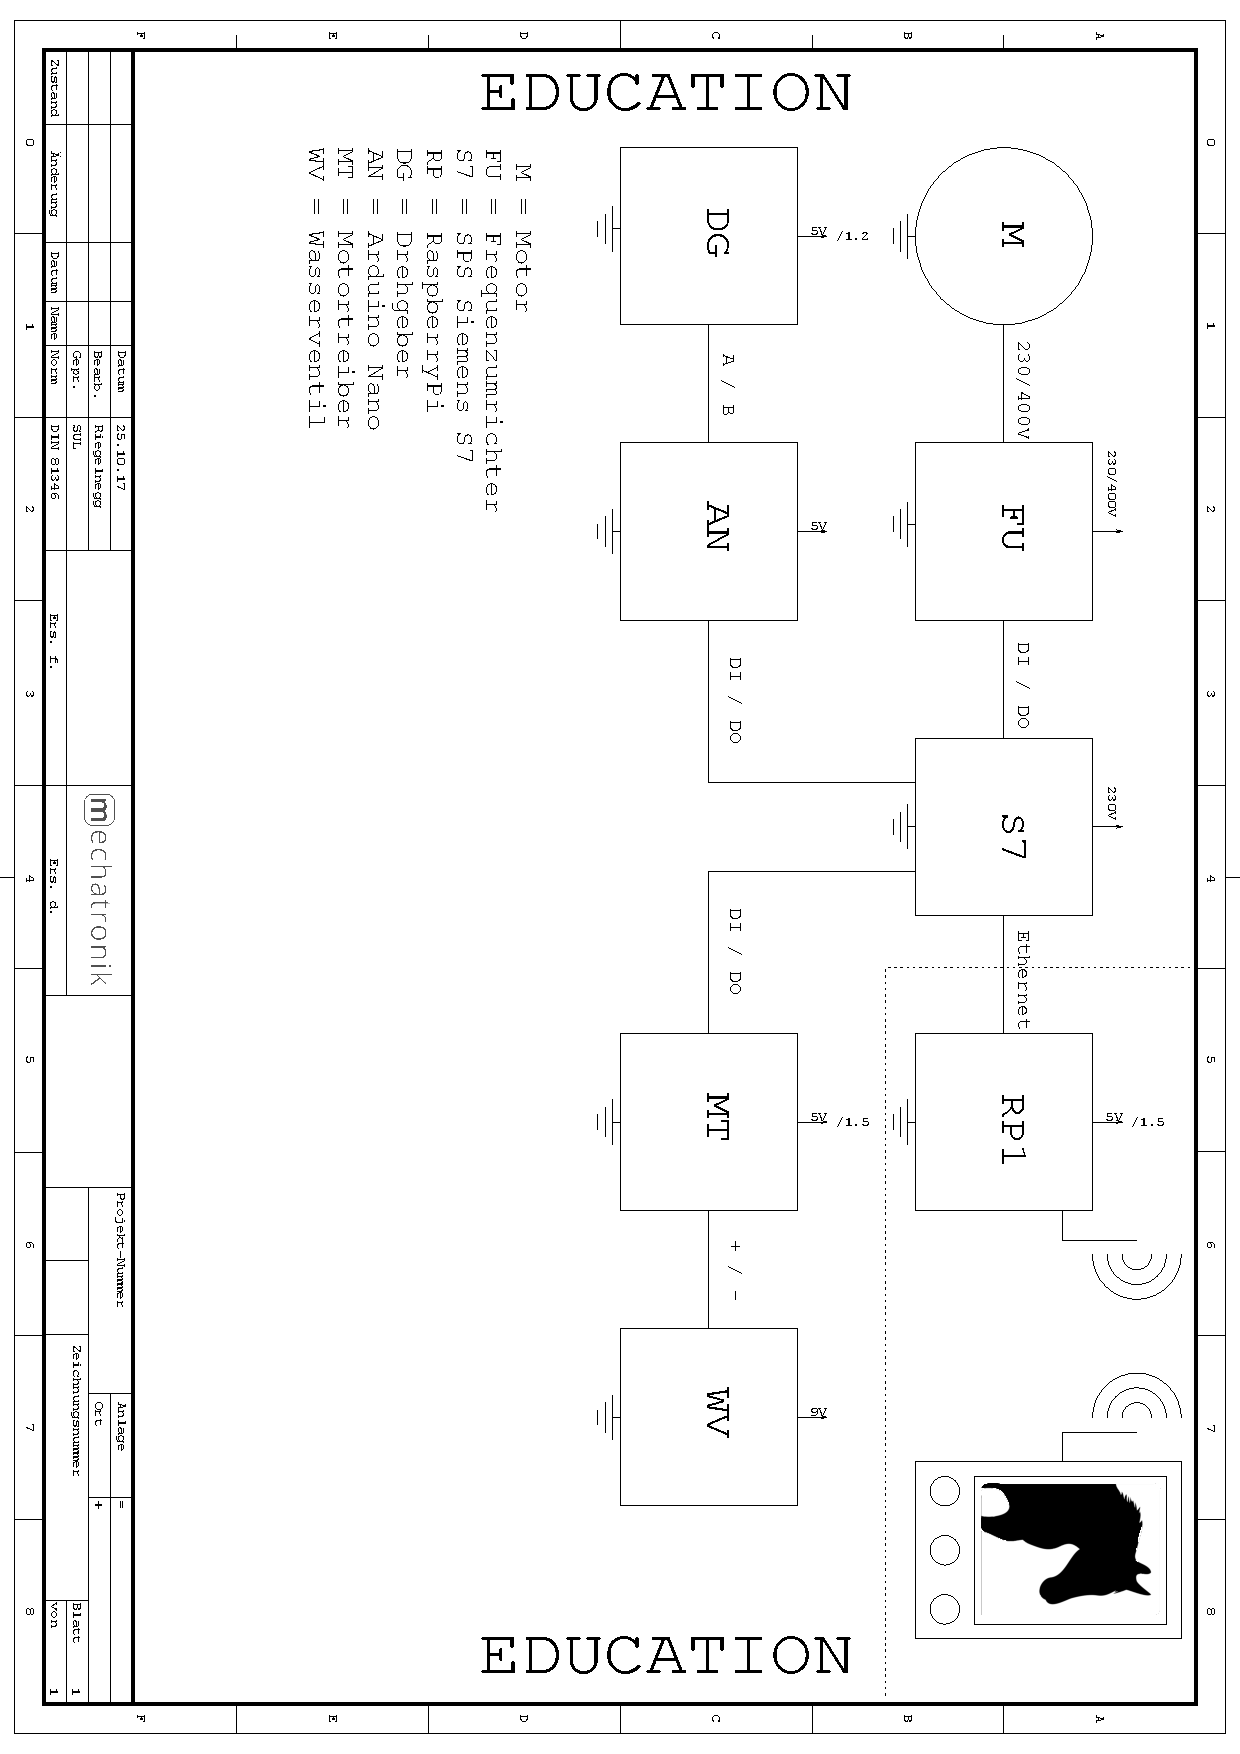
\includegraphics[scale=0.86]{fig/Blockschaltbild1}

\markboth{}{}	%end chapter

\bibliography{Literaturverzeichnis}
\bibliographystyle{unsrt}

\chapter{Abkürzungsverzeichnis}
\begin{acronym}
%Abkürzung hinzufügen: \acro{Kürzel}{Ausgeschrieben}
	\acro{FU}{Frequenzumrichter}
	\acro{ISR}{Interrupt Service Routine}
	\acro{UART}{Universal Asynchronous Receiver and Transmitter}
	\acro{USB}{Universal Serial Bus}
	\acro{SPS}{Speicherprogrammierbare Steuerung}
\end{acronym}

\listoffigures
\listoftables
\lstlistoflistings													%Datei importieren
\end{document}